\documentclass{article}
\usepackage{amsmath}
\newcommand{\myvec}[1]{\ensuremath{\begin{pmatrix}#1\end{pmatrix}}}
\newcommand{\mydet}[1]{\ensuremath{\begin{vmatrix}#1\end{vmatrix}}}
\newcommand{\solution}{\noindent \textbf{Solution: }}
\providecommand{\brak}[1]{\ensuremath{\left(#1\right)}}
\providecommand{\norm}[1]{\left\lVert#1\right\rVert}
\let\vec\mathbf
\usepackage{float}
\usepackage{graphicx}
\title{Ch - 7 Coordinate geometry}
\author{Mahapatra Sampada(mahapatra.sampada@sriprakashschools.com)}
\date{1 August 2023}
\begin{document}
\maketitle
\section*{Class10${th}$ Maths- chapter 7}
This is problem 3 of exercise 7.3
\begin{enumerate}
\item Find the area of a triangle formed by joining the mid points of the sides of the triangle whose vertices are (0,-1) , (2,1) and (0,3). Find the ratio of this area to the area of the given triangle. \\

\solution\\
Let the points be A(0,-1) , B(2,1) , C (0,3)\\ 
\begin{align}
\vec{A}&=\myvec{0\\-1}\\
\vec{B}&=\myvec{2\\1}\\
\vec{C}&=\myvec{0\\3}\\
\end{align}
Let $\vec{D}$,$\vec{E}$,and $\vec{F}$ be the midpoints of $\vec{AB}$, $\vec{BC}$ and $\vec{CA}$
\begin{align}
    \vec{D} &= \frac{(1)\vec{B}+(1)\vec{A}}{2}\\
    \vec{D} &= \frac{(1)\myvec{2\\1}+(1)\myvec{0\\-1}}{2}\\
    \vec{D} &= \frac{\myvec{2\\0}}{2}\\
    \vec{D} &= \myvec{1\\0}\\
    \vec{E} &= \frac{(1)\vec{C}+(1)\vec{B}}{2}\\
    \vec{E} &= \frac{(1)\myvec{0\\3}+(1)\myvec{2\\1}}{2}\\
    \vec{E} &= \frac{\myvec{2\\4}}{2}\\
    \vec{E} &= \myvec{1\\2}\\
    \vec{F} &= \frac{(1)\vec{A}+(1)\vec{C}}{2}\\
    \vec{F} &= \frac{(1)\myvec{0\\-1}+(1)\myvec{0\\3}}{2}\\
    \vec{F} &= \frac{\myvec{0\\2}}{2}\\
    \vec{F} &= \myvec{0\\1}\\
\end{align}
Area of triangle ABC=
 \begin{align}
 &=\frac{1}{2}\norm{\vec{AB}\times\vec{AC}}\\
  &=\frac{1}{2}\mydet{2&0\\2&4}\\
   &=\frac{1}{2}\norm{8}\\
    &=4 sq.units\\
\end{align}
Area of triangle DEF= 
 \begin{align}
 &=\frac{1}{2}\norm{\vec{DE}\times\vec{DF}}\\
  &=\frac{1}{2}\mydet{0&-1\\2&0}\\
   &=\frac{1}{2}\norm{2}\\
    &=1 sq.units\\
 \end{align}
 Therefore, the ratio between the triangle DEF and ABC = 1:4
\end{enumerate}
\begin{figure}[H]
			\centering
			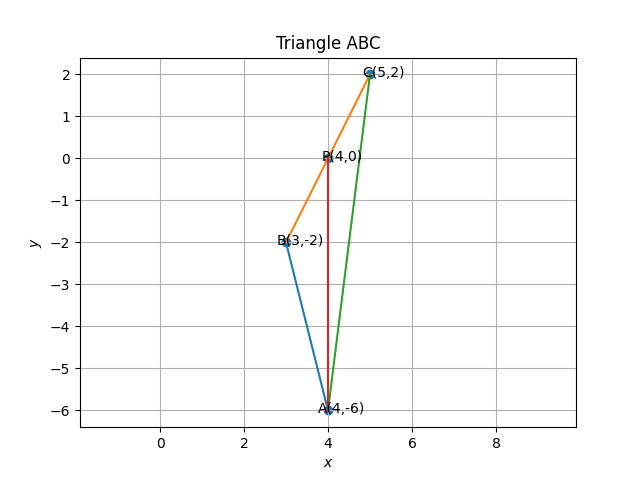
\includegraphics[width=\columnwidth]{figs/Figure_1.png}
			\caption{Triangles ABC and DEF}
			\label{fig:tri2}
		\end{figure}
\end{document}
